\documentclass[12pt]{article}
\usepackage{amsmath}
\usepackage{amsfonts}
\usepackage{amssymb}
\usepackage{graphicx}
\usepackage{hyperref}
\usepackage{geometry}
\usepackage{amsmath}
\geometry{margin=1in}

\title{Linear Algebra and Differential Equations Project 1}
\author{Rayana Gottschall}
\date{\today}

\begin{document}

\maketitle
%\tableofcontents
\newpage

\section*{Abstract}
[Write a brief summary of your project here.]

\section{Part 1: Colley Method}
\subsection{Explanation}
Colley's method is used to rank sports teams based on their win-loss ratio.
The method was created by Wesley Colley to handle situations where teams may 
not have played each other an equal number of times. Colley's method takes advantage
of Laplace's Rule of Succession.
\begin{center}
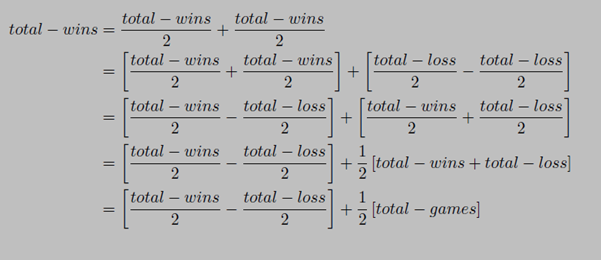
\includegraphics[width=0.8\textwidth]{colleysmethod.png}
\end{center}

\subsection{Laplace's Rule of Succession}
Laplace's Rule of Succession provides a formula to relate observed 
instances to unobserved ones, formally reffered to as "enumerative induction." 
The formula for probability is (k+1)/(n+2). Where 'k' is the number of times an 
event has occured, and 'n' is the total number of trials. 
In sports ranking, Laplace's rule provides a more accurate probabilty result for small data
 sets by accounting for future outcomes. 
This is acheieved through the use of biases, +1 and +2. 
The bias also eases the jumps in ranking when the observed data, number of games played, is
 scarce.


\subsection{Example Calculation}
[Provide a sample calculation to illustrate the method.]

\section{Part 2: Massey Method}
\subsection{Introduction}
Massey's method includes teams' differences in points, and assumes transitivity 
will hold true. 

\subsection{Methodology}
[Explain the approach and relevant equations.]

\subsection{Example Calculation}
[Show an example using the method.]

\subsection{Results}
[Discuss your findings from applying the Massey method.]

\section{Part 3: Application to Real Data}
\subsection{Data Collection}
[Explain the source and characteristics of the data you used.]

\subsection{Implementation}
[Discuss how you applied the Colley and Massey methods to the real data.]

\subsection{Comparison of Results}
[Compare the outcomes of both methods when applied to the data.]

\section{Part 4: Cutting Edge}
\subsection{Overview of New Methods}
[Summarize any novel or emerging methods in ranking.]

\subsection{Application and Analysis}
[Describe your research and analysis of the cutting-edge approach.]

\subsection{Bayesian Analysis of Formula One race Results}
Unlike football and basketball, Formula One racing has an additional factor: the car.
Each Formula One team has its own unique car, because of this, in what way can we compare
driver skill? The Bayesian Analysis mathematics proposed by Kesteren and Bergkamp uses driver data 
from 2014-2021 and the attributes are as follows: driver id, constructor id, season, race number, 
finishing position, and status. Additional race information included weather conditions (ie wet 
or dry) and circuit type (street or permanent).

\subsubsection{Diving into the Math}
For each race, r, we assume there is a set of competitors, C. The outcome is a vector which 
represents a ranking of competitors, y. The ranking follows a Rank-Ordered Logit model where 
finish position (ranking) is modeled as a function of driver skill, constructor advantage, and 
yearly variations in performance.

Rank-Ordered Logit:
\[
\mathbf{y}_r \sim \text{RankOrderedLogit}(\boldsymbol{\theta}_r)
\]
where \(\boldsymbol{\theta}_r\) represents the latent abilities of competitors in race \(r\).

Latent Ability Decomposition: 
the ability of a competitor is decomposed into the following components
\[
\theta_c = \theta_d + \theta_{ds} + \theta_t + \theta_{ts}
\]
\[
\begin{aligned}
&\theta_d \text{: Long-term driver skill,} \\
&\theta_{ds} \text{: Seasonal deviation of driver skill,} \\
&\theta_t \text{: Long-term constructor advantage,} \\
&\theta_{ts} \text{: Seasonal deviation of constructor advantage.}
\end{aligned}
\]



\begin{center}
    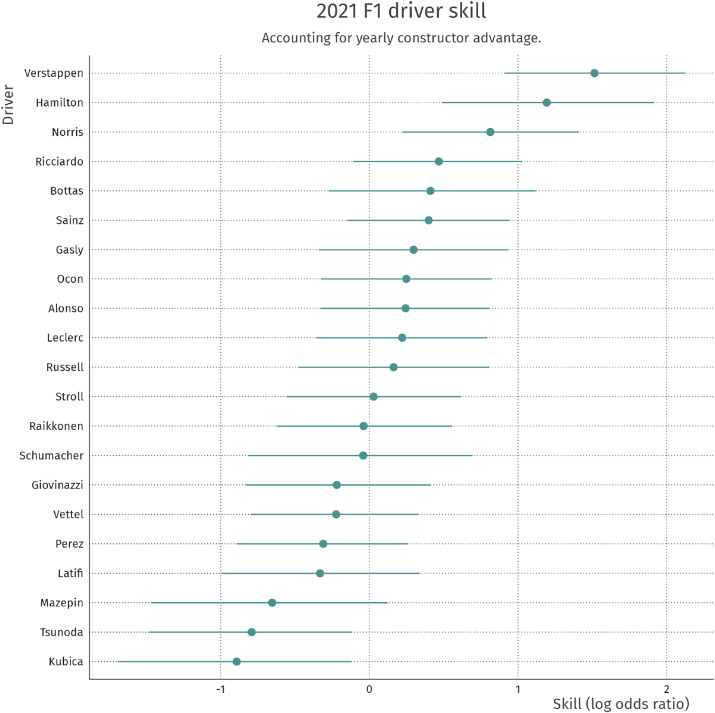
\includegraphics[width=0.8\textwidth]{driver skill.jpg}
    \end{center}

\newpage
\section*{References}
[Include your references here in the format required by your institution.]

\end{document}
